\documentclass[a4paper,UKenglish]{lipics-v2016}

\usepackage{upquote}
\usepackage{microtype}
\usepackage{pifont}
\usepackage{fp}
\usepackage{graphicx}
\usepackage{semantic}
\usepackage{lipsum}

\bibliographystyle{plainurl}

% ==================================================================================================

\title{Data exploration through dot-driven development (artifacat evaluation)}
\titlerunning{Data exploration through dot-driven development}

\author[1]{Tomas Petricek}
\affil[1]{The Alan Turing Institute, London, UK\\
  \texttt{tomas@tomasp.net}}
\authorrunning{T. Petricek}
\Copyright{Tomas Petricek}
\subjclass{D.3.2 Very high-level languages}
\keywords{Data science, type providers, pivot tables, aggregation}


\EventEditors{John Q. Open and Joan R. Acces}
\EventNoEds{2}
\EventLongTitle{42nd Conference on Very Important Topics (CVIT 2016)}
\EventShortTitle{DRAFT}
\EventAcronym{DRAFT}
\EventYear{2016}
\EventDate{December 24--27, 2016}
\EventLocation{Little Whinging, United Kingdom}
\EventLogo{}
\SeriesVolume{42}
\ArticleNo{23}

% ==================================================================================================

\theoremstyle{plain}
\theoremstyle{definition}
\newtheorem{rmrk}{Remark}

% Formatting for source code & types
\definecolor{cmtclr}{rgb}{0.0,0.6,0.0}
\definecolor{kvdclr}{rgb}{0.0,0.0,0.6}
\definecolor{numclr}{rgb}{0.0,0.4,0.0}
\definecolor{strclr}{rgb}{0.4,0.3,0.0}
\definecolor{prepclr}{rgb}{0.6,0.0,0.2}

\newcommand{\vect}[1]{\langl #1 \rangl}
\newcommand{\langl}{\begin{picture}(4.5,7)
\put(1.1,2.5){\rotatebox{60}{\line(1,0){5.5}}}
\put(1.1,2.5){\rotatebox{300}{\line(1,0){5.5}}}
\end{picture}}
\newcommand{\rangl}{\begin{picture}(4.5,7)
\put(.9,2.5){\rotatebox{120}{\line(1,0){5.5}}}
\put(.9,2.5){\rotatebox{240}{\line(1,0){5.5}}}
\end{picture}}

\newcommand{\ball}[1]{\FPeval{\result}{clip(201+#1)}\textnormal{\ding{\result}}}

\newcommand{\lsep}{~\,|\,~}
\newcommand{\num}[1]{\textcolor{numclr}{#1}}
\newcommand{\str}[1]{\textnormal{\textcolor{strclr}{\sffamily "#1"}}}
\newcommand{\kvd}[1]{\textnormal{\textcolor{kvdclr}{\sffamily #1}}}
\newcommand{\ident}[1]{\textnormal{\sffamily #1}}
\newcommand{\qident}[1]{\textnormal{\sffamily \guillemotleft #1\guillemotright}}
% \newcommand{\qident}[1]{\textnormal{\sffamily ‹#1›}}

\newcommand{\dom}{\ident{dom}}

% ==================================================================================================

\begin{document}
\maketitle

% ==================================================================================================

~

~

\section{Installation instructions}

The tool implemented as part of the submitted paper is available as a JavaScript library that
parses, type-checks and runs sample scripts and creates an editor that can be used for writing
code in the browser. The library calls a server to evaluate queries constructed using the pivot
type provider.

The presented artifact consists of a simple web server packaged as a Docker container. When 
started, the web server hosts the service that provides data to the web browser, as well as
a sample web page with a number of demos illustrating the language.

To run the artifact, you will need to install Docker (\url{https://www.docker.com}) and the
Google Chrome browser (\url{http://www.google.co.uk/chrome}) and also download the provided
docker image \texttt{thegamma-ecoop17.tar}. Next, use the \texttt{docker load} command to 
unpack the image and \texttt{docker run} to start the web server:

\begin{verbatim}
    docker load --input thegamma-ecoop17.tar
    docker run -p 8889:80 thegamma-ecoop17
\end{verbatim}

\noindent
Alternatively, the \texttt{thegamma-ecoop17} Docker image is also hosted on the Docker repository
and can be downloaded and executed directly from the Docker repository:

\begin{verbatim}
    docker run -p 80:8889 tomasp/thegamma-ecoop17
\end{verbatim}

\noindent
The above commands specify the \texttt{-p 8889:80} parameter, which instructs Docker to map the
server hosted at port 80 inside the Docker container to a port 8889 of the host machine. Once
the Docker container starts, you will be able to access the sample web site by opening 
\url{http://localhost:8889} in the Google Chrome browser.

\begin{figure}[t]
\begin{center}
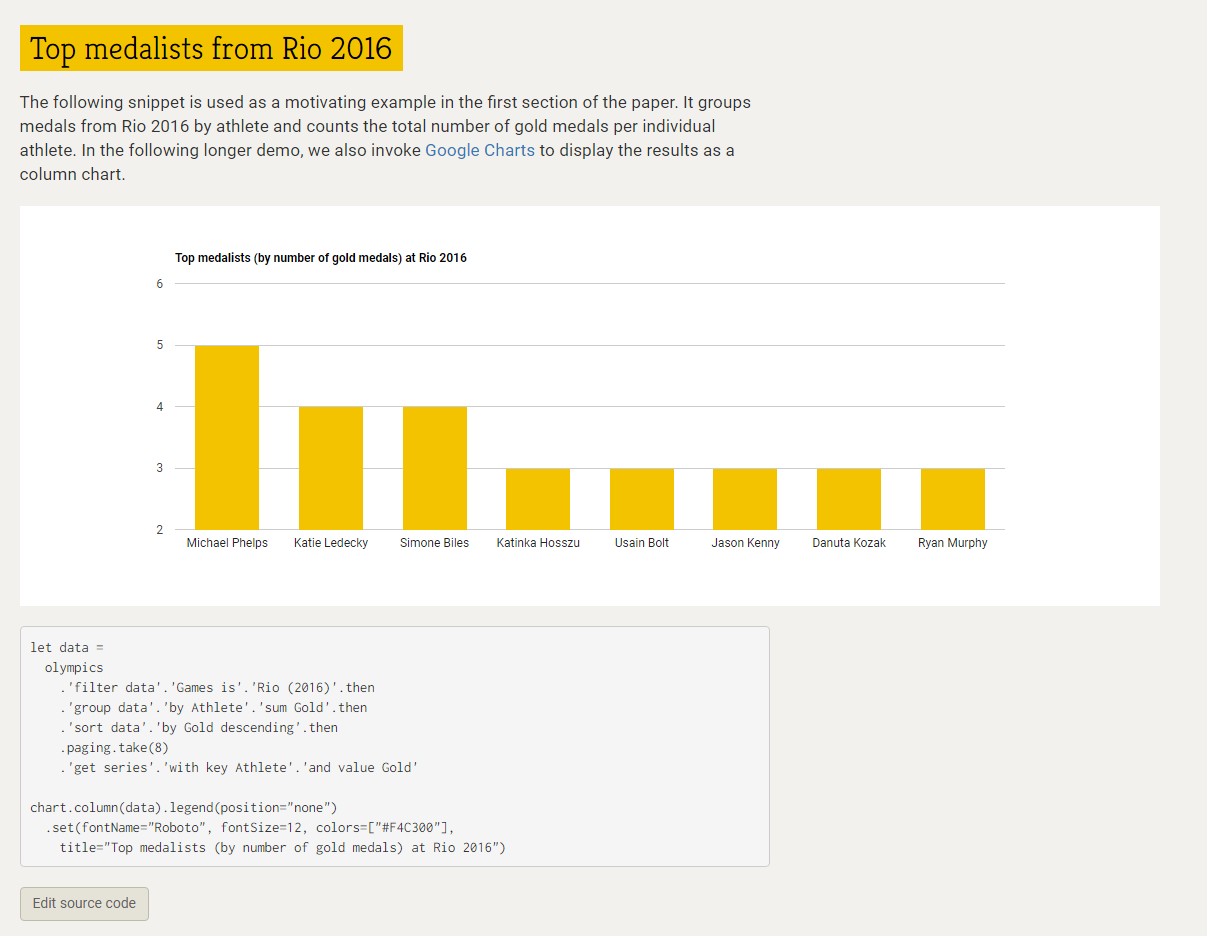
\includegraphics[scale=0.35,trim=0mm 0mm 0mm 0mm,clip]{images/af-preview.png}
\end{center}
\caption{Visualization showing top medalist from Rio 2016 with source code}
\label{fig:chart}
\end{figure}

\section{Exploring the examples}

The sample page contains a number of examples that illustrate the pivot type provider. When the
page loads, the examples are executed and the results appear as illustrated in Figure~\ref{fig:chart}.
For each example, the web page shows the full source code using the pivot type provider together
with several additional libraries not presented in the paper (such as \texttt{chart} and \texttt{table}),
which are used for creating visualizations.

Clicking on the ``Edit source code'' button opens an editor where the code can be modified. The
editor supports auto-completion, which is the key feature made possible by the type system of the
language and the pivot type provider. The following three sections briefly describe three scenarios
that illustrate interesting aspects of the artifact.

\begin{figure}
\begin{center}
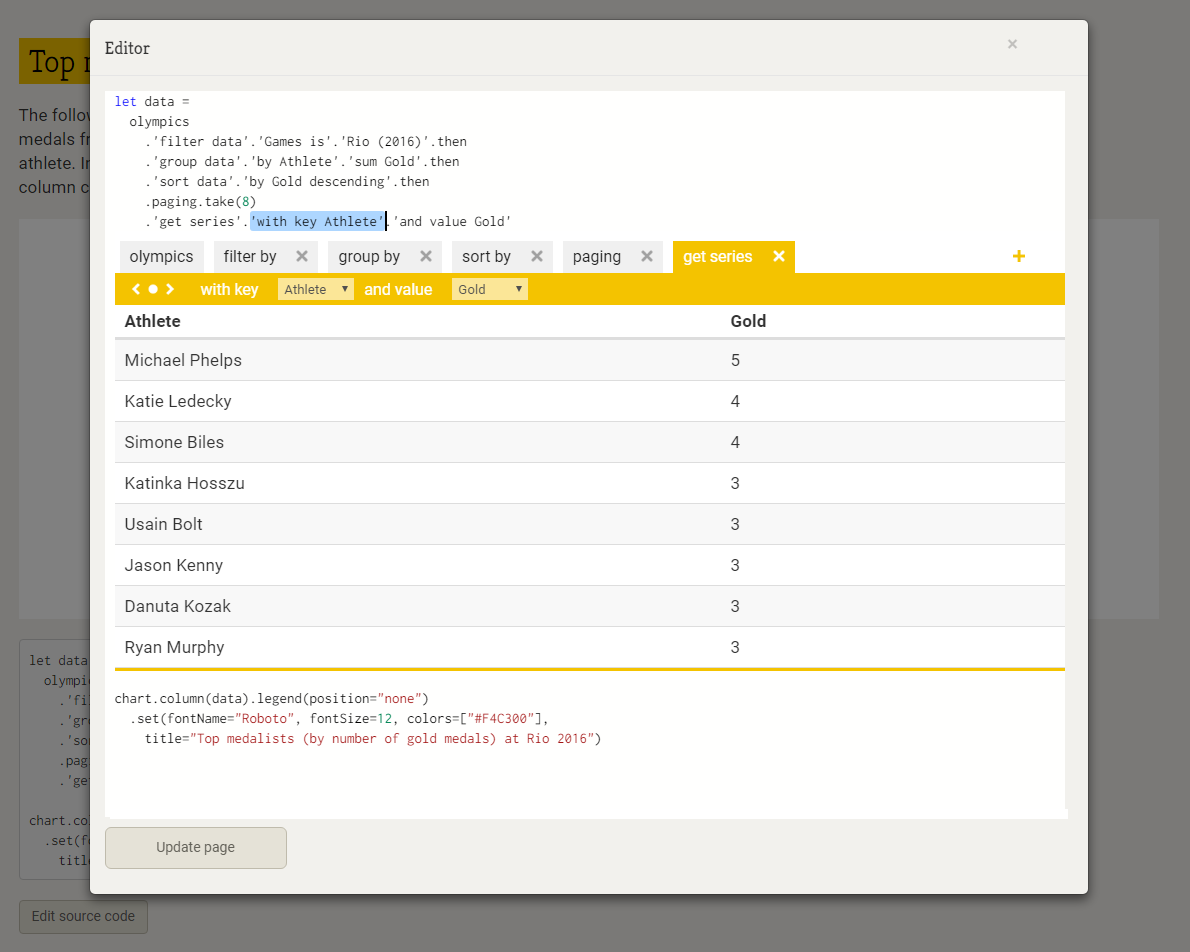
\includegraphics[scale=0.35,trim=0mm 0mm 0mm 0mm,clip]{images/af-editor.png}
\end{center}
\caption{Visualization showing top medalist from Rio 2016 with source code.}
\label{fig:code}
\end{figure}

~

\subsection{Demo: Obtain top medallists from London 2012}

In the first demo, we make a simple change to an existing source code to create a bar chart
showing top medallists from London 2012 rather than top medallists from Rio 2016.

\begin{enumerate}
\item Go to the first visualization ``Top medalists from Rio 2016'' and click the ``Edit source code''
  button to load the source code in the editor.
\item Locate the \texttt{Rio (2016)} member on the third line and delete it in the text editor.
  Additionally, delete the ``dot'' after \textt{Games is}.
\item Type ``.'' immediately after the quoted \texttt{Games is} member. An auto-complete list
  should appear showing the available Olympic games together with their years.
  Choose \texttt{London (2012)} and make sure the identifier is separated from the following
  \texttt{then} member with another ``dot''.
\item Click ``Update page''. The visualization on the original demo page should change to show
  the new chart.
\end{enumerate}

\subsection{Demo: Obtain Mongolian gold medalists in code} 

This demo illustrates the experience of writing code using the pivot type provider from scratch.
We start with an empty code editor, start writing code and use auto-complete to create a simple
query.

\begin{enumerate}
\item Click on the ``Edit source code'' button for any of the examples and delete all source code
  in the editor, so that we can start from empty file.
  
\item Type \texttt{olympics.} and note that auto-complete offers different data transformations 
  as documented in the paper. Start by choosing \textt{filter data}, followed by 
  \textt{Team is} and \texttt{Mongolia}. Finally, complete the filtering by choosing \texttt{then}.
  Typing ``dot'' again offers the list of all available transformations.

\item Complete the query by typing ``dot'' and selecting items from auto-complete. When auto-complete
  is displayed, you can navigate using arrow keys and filter items by typing substrings of the
  member names. As you type, you can see the data calculated so far in the preview below the
  current line.

\begin{verbatim}
  olympics.'filter data'.'Team is'.Mongolia.then
    .'filter data'.'Medal is'.Gold.then.'get the data'
\end{verbatim}
  
\item Now that the data query is written, complete the sample by creating a table to show the results.
  Wrap the code in the following (note that the code written in previous step needs to be indented):

\begin{verbatim}
  let altan = (...)
  table.create(altan)   
\end{verbatim}

\item When you place the cursor inside the \texttt{table.create} call, you should see table as a
  preview. Click ``Update page'' and you should see the new table appear in the original demo page.
\end{enumerate}

\subsection{Demo: Count medals per discipline using the pivot user interface}

This demo introduces the user interface built on top of the pivot type provider as mentioned in the
case study presented in the paper. We will use the user interface to construct a simple query that
finds the number of medals awarded per discipline and finds the disciplines with the largest number
of medals. To do this, we make small edits to the code and complete the rest of the work using
a simple user interface.

\begin{enumerate}
\item Go to the ``All time medalists table'' demo and click ``Edit source code''.
\item In the displayed source code, click anywhere inside the query that performs the data aggregatoion
  so that the user interface displayed in Figure~\ref{fig:code} appears.
\item Remove all the operations except for \texttt{group by} by clicking on the ``x'' button on 
  the right. Start from the last one and remove \texttt{get the data}, \texttt{paging},
  \texttt{get the data} and \texttt{sort by}. Now, remove all the calculated aggregations 
  by clicking on ``x'' buttons in the yellow toolbar. 
\item Change the grouping key by selecting \texttt{by Discipline} in the drop down
  showing \texttt{by Athlete}. Next, add aggregation \texttt{count all} by clicking on the 
  ``+'' button in the yellow toolbar.
\item Add \texttt{sort by} transformation by clicking on the yellow ``+'' in the tab panel showing
  a list of operations. Then add sorting key \texttt{by count descending} by clicking on the ``+''
  in the yellow toolbar.    
\item Finally, add the \texttt{get the data} transformation to obtain the data. The final source
  code should look as follows:
\begin{verbatim}
  let data =
    olympics
      .'group data'.'by Discipline'.'count all'.then
      .'sort data'.'by count descending'.then
      .'get the data'
  table.create(data)  
\end{verbatim}
\item Finally, click ``Update page'' and review the newly produced table in the main page. You should
  see athletics at the top with 3856 medals and Jeu de Paume at the bottom with just 3 medals.
\end{enumerate}


\end{document}
